\documentclass{article}
\usepackage{ucs} 
\usepackage{graphicx}
\usepackage[utf8x]{inputenc} % Включаем поддержку UTF8  
\usepackage[russian]{babel}

\begin{document}
\section{Введение}
\hspace{12pt} Эффект Мёссбауэра, или ядерный гамма-резонанс, заключается в резонансном поглощении ядром гамма-кванта, который был испущен таким же ядром при переходе из возбужденного состояния в основное.
\\
\indent По-видимому, это один из самых <<острых>> физических резонансов из наблюдаемых экспериментально. Действительно, добротность мёссбауэровского резонанса можно оценить через отношение естественной ширины $\Gamma$ 
гамма-перехода ядра к энергии E этого перехода. Для наиболее употребительного в мёссбауэровской спектроскопии гамма-перехода ядра $^{57}Fe$ из возбужденного состояния с энергией E = 14,413 кэВ (период полураспада - 98,1 нс, $\Gamma$ $\approx$ $7\cdot 10^{-9}$ эВ) в основном добротность резонанса достигает величины $1,5\cdot 10^{12}$. В исключительных же случаях добротность мёссбауэрского резонанса оценивается величиной $10^{15}$ для $^{67}Zn$ и даже  $2\cdot 10^{22}$ для $^{107}Ag$. Именно в силу своей высокой добротности мёссбауэровский ядерный гамма-резонанс оказался мощным, а иногда и единственным методом измерения сверхмалых сдвигов энергии ядерных гамма-переходов.
\\
\indent Эффект Мёссбауэра лежит в основе мёссбауэровской спектроскопии, которая является неразрушающим методом исследования химического состава, кристаллической структуры и магнитных свойств конденсированного состояния вещества. Другое название этого метода исследования вещества - ядерная гамма-резонансная спектроскопия, или ЯГР-спектроскопия. Разумеется, с помощью мёссбауэровской спектроскопии можно исследовать только вещества, которые содержат ядра, демонстрирующие эффект Мёссбауэра, а этот эффект наблюдаем далеко не для всех ядер. Кроме того, это физическое явление может быть полезно для прецизионных измерений гамма квантов, например, с его помощью было измерено гравитационное смещение энергии фотонов.
\section{Физический смысл эффекта Мёссбауэра}
\hspace{12pt} Рассмотрим ядро $^{191}Ir$, находящееся в возбужденном состоянии с энергий E = 129 кэВ, из которого оно может перейти в основное состояние в результате испускания $\gamma$-кванта с периодом полураспада $T_{1/2} \approx 10^{-10}$сек. Тогда согласно соотношению неопределенностей энергия возбужденного состояния E известна с погрешностью $${\Delta}E \approx {\hbar}/{\Delta}t = \frac{10^{-27}}{10^{-10}\cdot 1,6 \cdot 10^{-12}} \approx 5 \cdot 10^{-6} \hspace{2pt}eV$$
\hspace{12pt}Чем быстрее происходит высвечивание возбужденного состояния, тем больше неопределенность в значении энергии возбужденного состояния. Только основное состояние стабильного ядра имеет $\Delta$E = 0 и, следовательно, характеризуется строго определенным значением энергии.
\\
\indent Неопределенность в энергии возбужденного состояния приводит к немонохроматичности $\gamma$-излучения, испускаемого при переходе ядра из возбужденного состояния в основное. Эту немонохроматичность принято называть естественной шириной $\Gamma$ линии испускания $\gamma$-излучения. В нашем примере $\Gamma \approx 5\cdot 10^{-6}$ эВ. Это очень малая величина по сравнению с энергией $\gamma$-перехода E = 129 кэВ. Поэтому если бы существовал способ обнаружения изменения энергии на величину порядка естественной ширины линии излучения, то он дал бы возможность измерять энергию с очень высокой относительной точностью, равной $\Gamma/E$. В нашем примере $\Gamma/E = 4\cdot 10^{-11}$. Для более узких линий, т.е для $\gamma$-переходов с большими периодами, значение $\Gamma/E$ должно быть еще меньше.
\\
\indent В принципе обнаружить изменение энергии, равное естественной ширине линии излучения, можно при помощи резонансного поглощения $\gamma$-излучения. Резонансным поглощением $\gamma$-излучения называется процесс возбуждения ядра под действием $\gamma$-квантов, испускаемых этими ядрами при обратных переходах и данного возбужденного состояния в основное.
\\
\indent Процесс резонансного поглощения можно сравнительно легко наблюдать экспериментально, изучая прохождение резонансного $\gamma$-излучения через пластинку из данного вещества. При совпадении энергии $\gamma$-излучения с энергией перехода поглощение резко возрастает, что позволяет заметить очень небольшие изменения энергии вблизи резонансного значения. Однако до 1958 г. этот метод можно было использовать только при достаточно больших ширинах линий.
\\
\indent Дело в том, что при переходе ядра из возбужденного состояния с энергией E в основное состояние испускающийся $\gamma$-квант уносит не всю энергию возбуждения E, а несколько меньшую величину $E_{\gamma_{em}}$, так как часть энергии $T_{nuc}$ идет на отдачу испускающего ядра: 
$$ E_{\gamma_{em}} = E - T_{nuc} < E$$
(сравните с аналогичным явлением в $\alpha$- и $\beta$-распаде).Аналогично для возбуждения ядра до энергии E необходимо $\gamma$-излучение с энергией 
$$ E_{\gamma_{abs}} = E + T_{nuc} > E,$$
где $T_{nuc}$ - энергия отдачи, передаваемая $\gamma$-квантом поглощающему ядру. Таким образом, линия испускания и линия поглощения для одного и того же состояния в данном ядре сдвинуты относительно друг друга на 2$T_{nuc}$

\begin{figure}[h]
\center{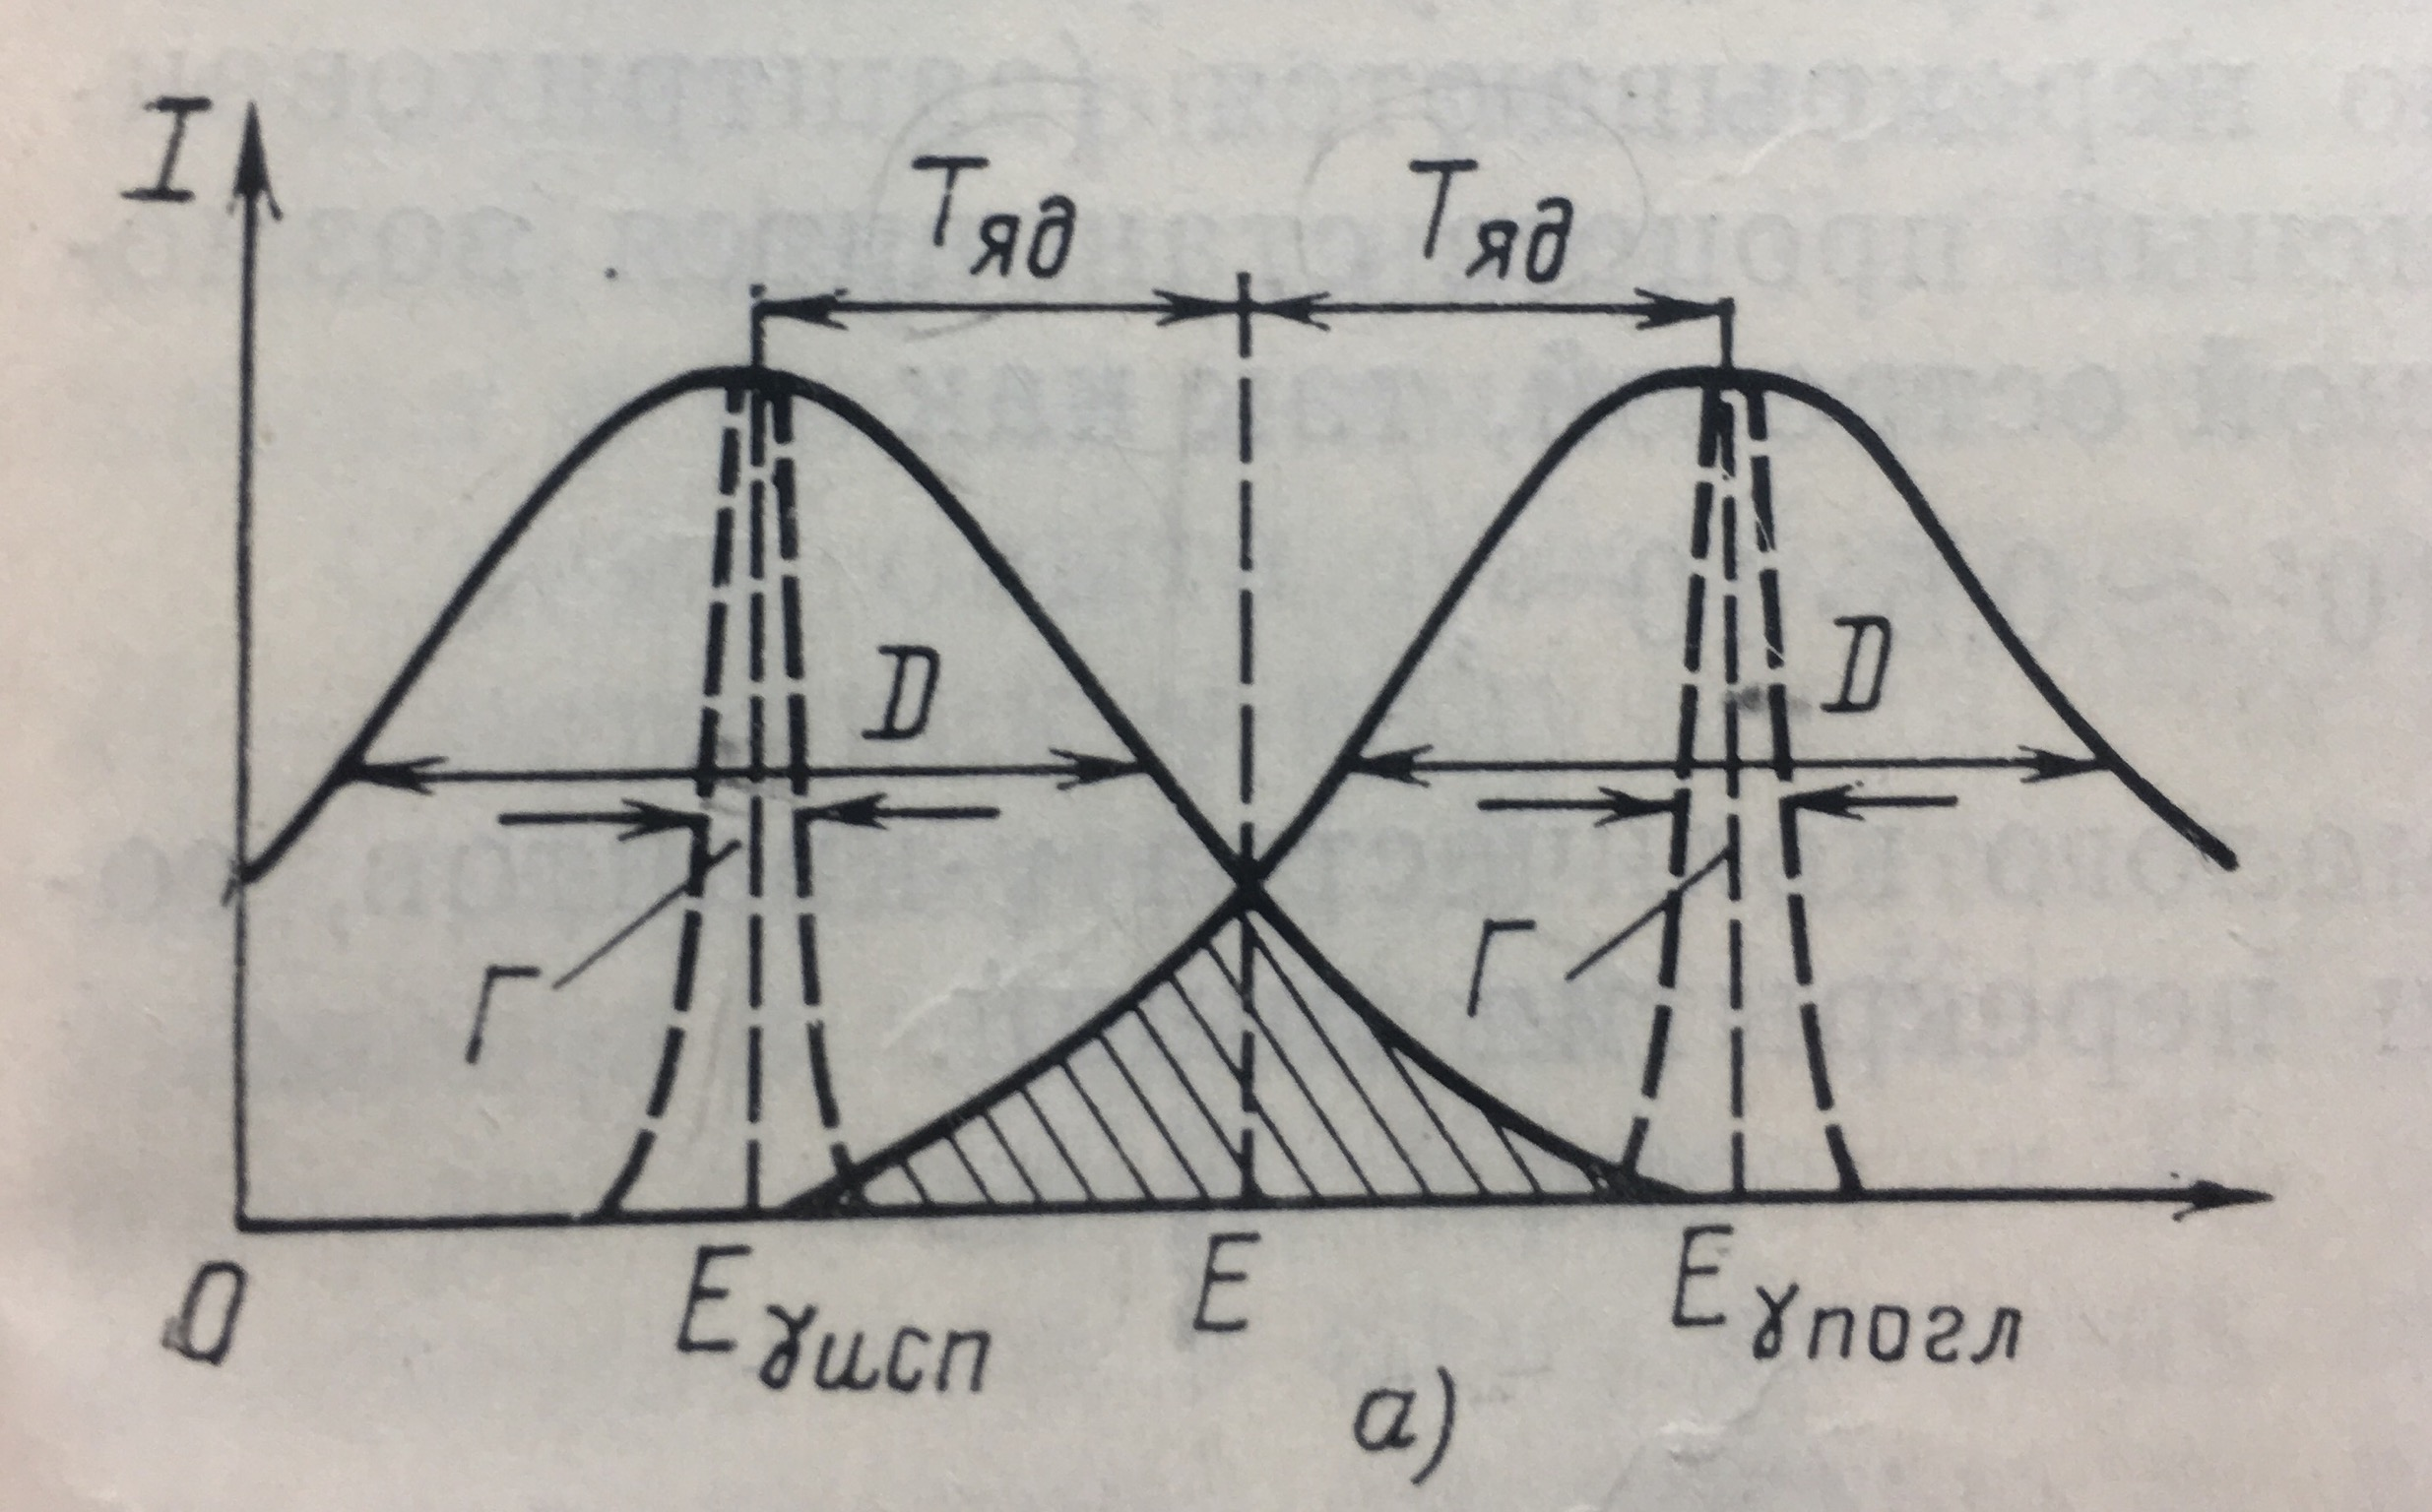
\includegraphics[scale=0.05]{a.jpg}}
\caption{сдвиг}
\label{fig:image}
\end{figure}

\indent Энергию отдачи легко подсчитать, если учесть, что в процессе испускания $\gamma$-кванта должен выполняться закон сохранения импульса $p_{\gamma}$ = $p_{nuc}$:
$$ T_{nuc} = P_{nuc}^{2}/2M_{nuc} = p_{\gamma}^{2}/2M_{nuc} = E_{\gamma}^{2}/2M_{nuc}c^{2} \approx E^{2}/2M_{nuc}c^{2}.$$
\indent Для нашего примера получается очень небольшое значение
$$ T_{nuc} = (1,29\cdot 10^{5})^2/2\cdot 191 \cdot 931 \cdot 10^{6} \approx 0,05 \hspace{2pt}eV$$
однако оно существенно превышает естественную ширину линии излучения $\Gamma$:
$$ T_{nuc} \gg \Gamma $$
\indent Казалось бы отсюда следует абсолютная невозможность резонансного процесса. Однако это неверно потому, что реальная ширина линии испускания(и линии поглощения) определяется не естественной шириной $\Gamma$, а доплеровским уширением:
$$ D = 2\sqrt{T_{nuc}kT^0}$$,
которое при комнатной температуре (T = 300 K, kT = 0,025 эВ) равно
$$ D(300 \hspace{2pt}K) = 2\sqrt{0,05\cdot 0,025} \approx 0,07 \hspace{2pt} eV$$
\indent В связи с тем что $D \approx T_{nuc}$, доплеровски уширенные линии испускания и поглощения частично перекрываются (заштрихованная область на рисунке)  резонансный процесс становится возможен. Правда, он не обладает большой остротой, так как
$$ E/\Gamma = 0,07/1,3 \cdot 10^{5} \approx 0,5 \cdot 10^{-6},$$
и наблюдается только для очень малого количества $\gamma$-квантов, соответствующих небольшой области перекрытия линий.

\section{Два опыта Мёссбауэра}
\hspace{12pt} В 1958 г. немецкий физик Р. Мёссбауэр, проводя опыты по изучению резонансного поглощения в условиях частичного перекрытия линий в результате их доплеровского уширения, решил уменьшить D при помощи охлаждения источника и поглотителя. При этом естественно было ожидать уменьшения доли поглощенных квантов (из-за сокращения области перекрытия линий). Вместо этого в опыте было обнаружено увеличение эффекта, которое свидетельствовало о возрастании области перекрытия.
\indent Для объяснения этого странного результата Мёссбауэр предположил, что при определенных условиях (достаточно малая энергия перехода и низкая температура по сравнению с дебаевской температурой кристалла) импульс и энергия отдачи, возникающие при испускании (поглощении) $\gamma$-кванта, не идут ни на выбивание атома из узла решетки, ни на изменение энергетического состояния кристалла, а передаются упругим образом всему кристаллу в целой (точнее, очень большой группе атомов - $N \approx 10^{8}$, охватываемой бегущей звуковой волной за время испускания). В этом случае корреляция между импульсом и энергией ядра-излучателя (поглотителя) разрывается, так как из-за большой массы кристалла энергия отдачи R практически равна нулю:
$$ R = P_{nuc}^{2}/2 \cdot 10^{8} \cdot M_{nuc} = T_{nuc}/10^{8} \approx 5 \cdot 10^{-10} \hspace{2pt} eV \ll \Gamma $$
\indent В результате становятся возможными акты испускания (поглощения) $\gamma$-квантов без отдачи, т.е. сдвиг между линией испускания и линией поглощения исчезнет,
$$ E_{\gamma_{em}} = E_{\gamma_{abs}} .$$
\indent Одновременно для этих актов испускания и поглощения должно исчезнуть и доплеровское уширения D, которое теперь будет меньше естественной ширины линии $\Gamma$,
$$ D(88K) = 2\sqrt{RkT_{88^{\textdegree}}} = 2\sqrt{5 \cdot 10^{-10} \cdot 0,0075} \approx 4 \cdot 10^{-6} \hspace{2pt}eV < \Gamma$$
\indent Другими словами, при перечисленных выше условиях должен наблюдаться острый резонанс без отдачи с шириной, равной естественной ширине линии $\Gamma$. Это объяснение Мёссбауэр блестяще доказал в своем знаменитом втором опыте.
\\
\indent Схема опыта Мёссбауэра изображена на рисунке. Здесь И - источник $\gamma$-излучения $^{191}Ir$ с энергией 129 кэВ, П - иридиевый поглотитель, Д - детектор. Источник и поглотитель были помещены в криостаты $K_1$ и $K_2$, в которых поддерживалась температура T = 88 K. Криостат $K_2$ с источником мог вращаться. При вращении его в одну сторону источник приближался в поглотителю с некоторой скоростью $\vartheta$, а при вращении в другую сторону удалялся от него с той же скоростью.

\begin{figure}[h]
\center{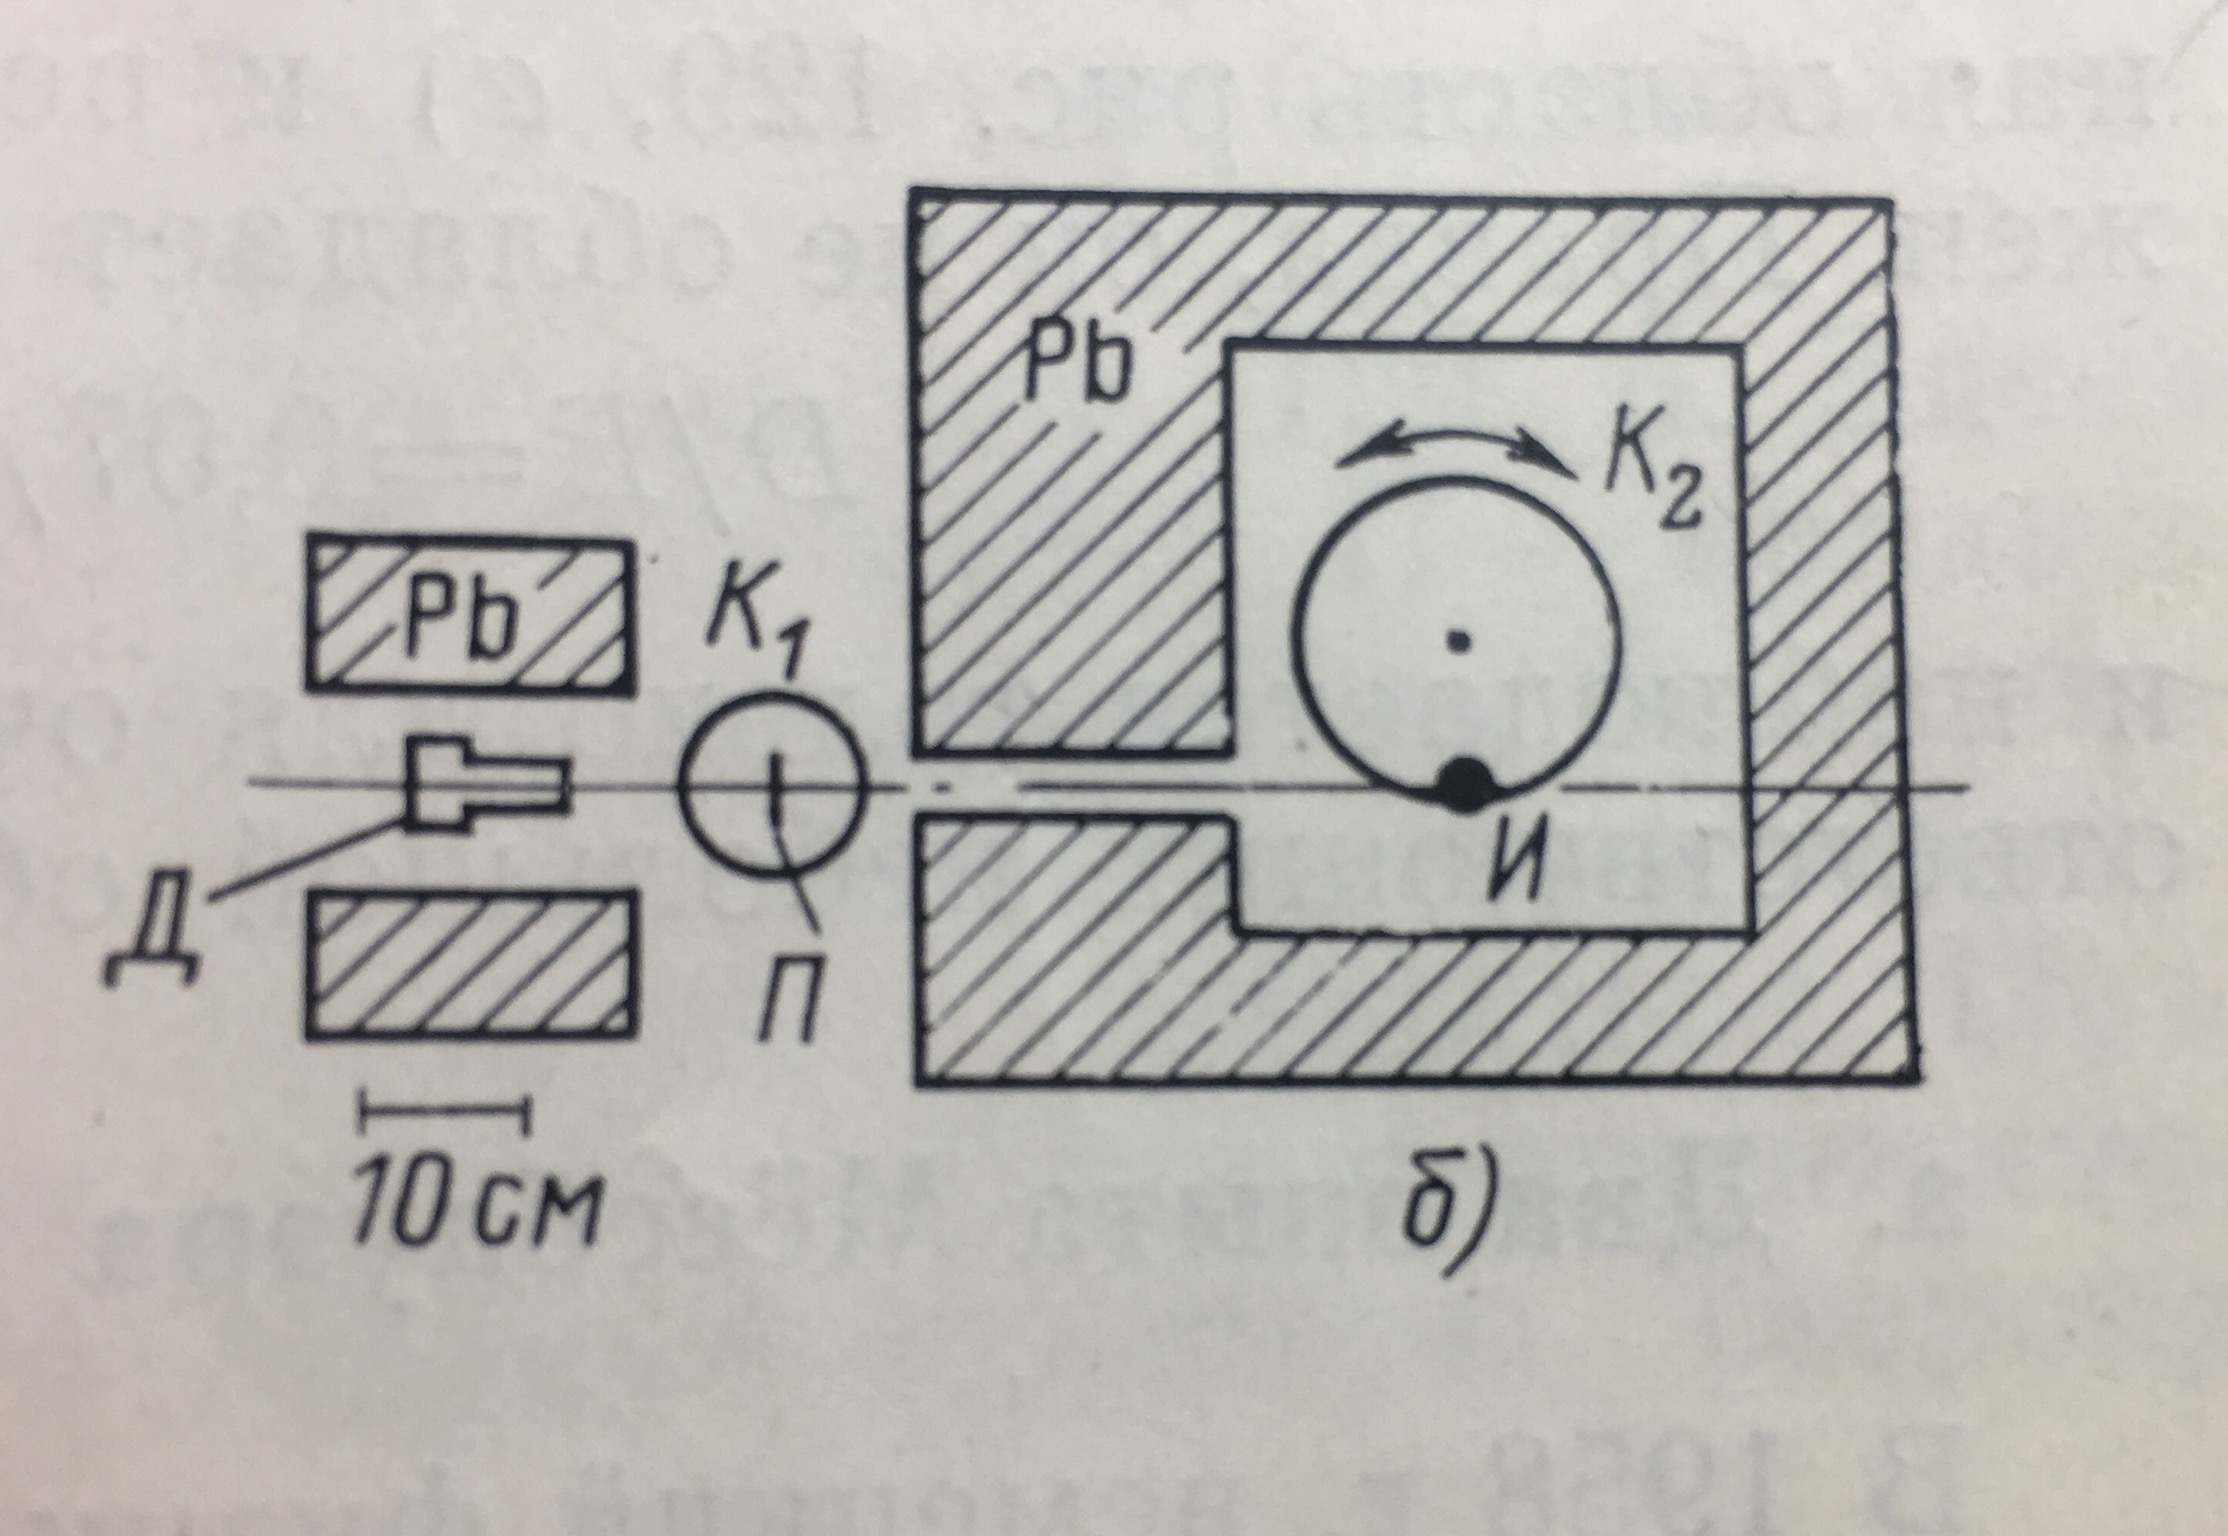
\includegraphics[scale=0.05]{b.jpg}}
\caption{Схема опыта Мёссбауэра}
\label{fig:image}
\end{figure}

\indent В опыте измерялось поглощение $\gamma$-квантов при различных скоростях источника. Результаты опыта приведены на рисунке.
\\
\indent Здесь по оси абсцисс отложена относительная скорость источника и поглотителя и соответствующие ей изменение энергии $\Delta E$ испускаемых $\gamma$-квантов (из-за эффекта Доплера). По оси ординат отложена относительная разность интенсивности $\gamma$-излучения, проходящего через иридиевый и платиновый (для оценки фона) поглотители одинаковой толщины. Из рисунка видно, что резонанс нарушается уже при скоростях в несколько сантиметров в секунду, которые соответствуют доплеровскому изменению энергии $\gamma$-квантов, меньшему $10^{-5} \hspace{2pt}eV$. Отсюда следует, что в опыте действительно наблюдалась линия без отдачи с естественной шириной ${\gamma}$-перехода, равной $\Gamma \approx 5\cdot 10^{-6} \hspace{2pt} eV$

\begin{figure}[h]
\center{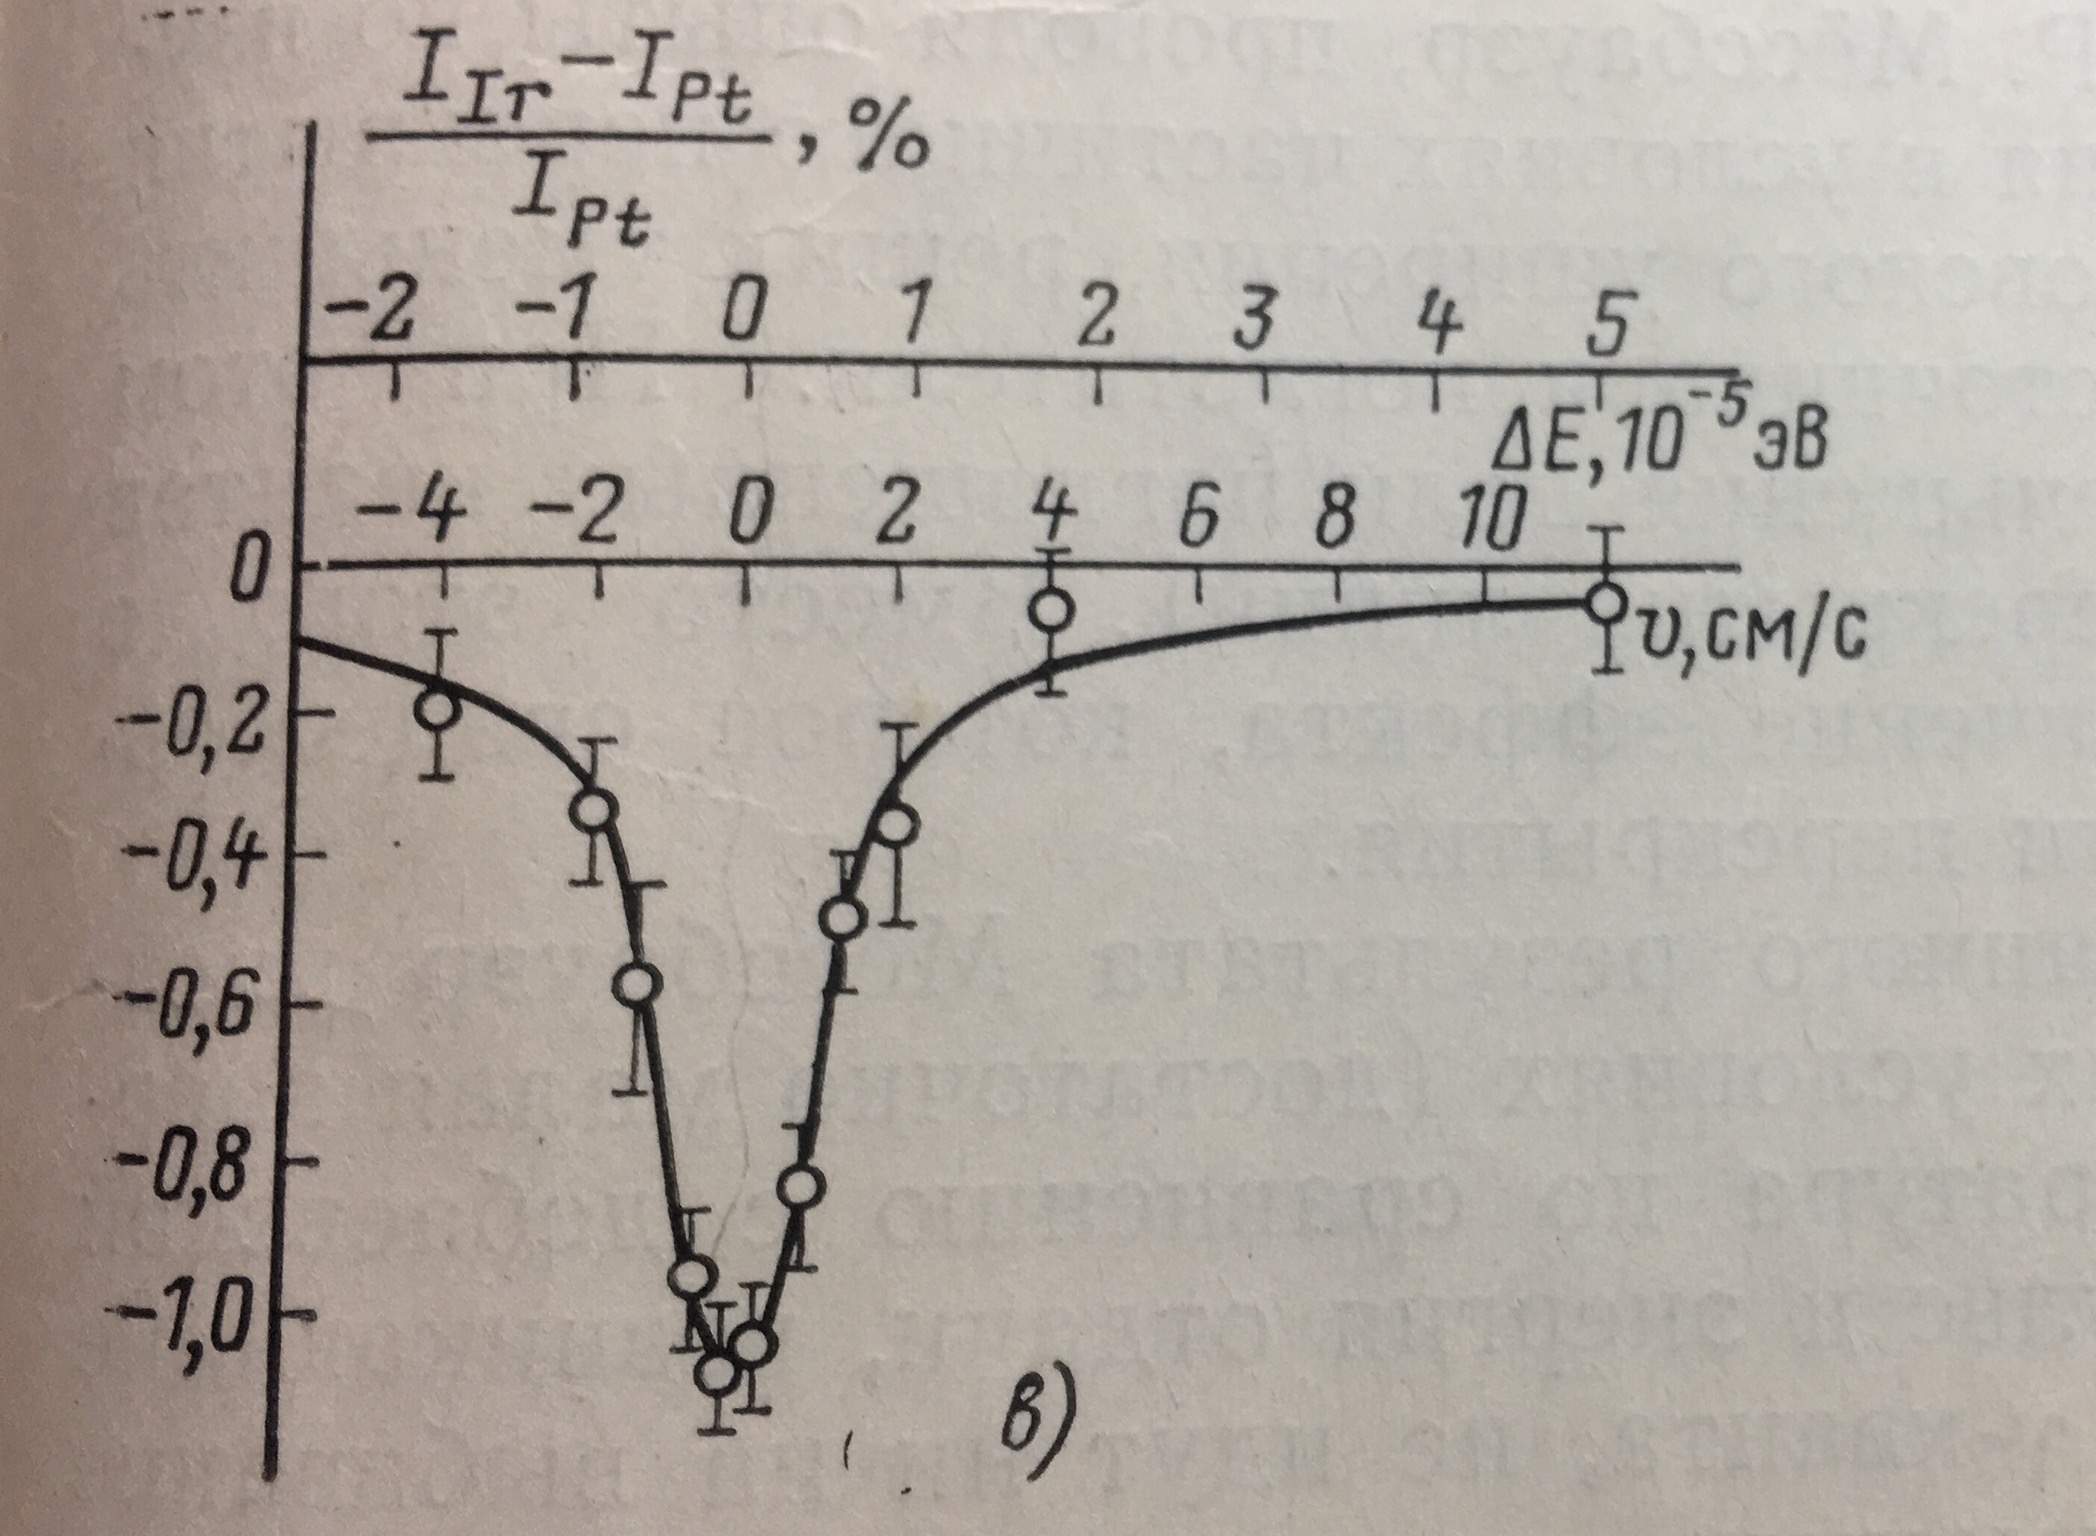
\includegraphics[scale=0.05]{c.jpg}}
\caption{Результаты опыта Мёссбауэра}
\label{fig:image}
\end{figure}

\indent Метод резонансного поглощения позволяет измерять очень малые изменения энергии. Выше указывалось, что мерой точности этого метода может служить величина $\Gamma$/E, которая для рассмотренного примера равна $4\cdot10^{-11}$. На самом деле относительная точность измерения энергии еще выше, так как экспериментально можно заметить изменение поглощение при сдвиге линии на 1/100 долю от ее естественной ширины.
\\
\indent Эффект Мёссбауэра наблюдался для многих веществ, причем для некоторых из них были зарегестрированы еще более узкие линии. Величина эффекта бывает около 1$\%$, а иногда и еще меньше, рабочие температуры колеблются для разных веществ от комнатной до гелиевой (примерно 4 К). С ростом температуры эффект постепенно ослабевает и пропадает.
\\
\indent За открытие излучения, рассеяния и поглощения без отдачи Р. Мёссбауэру была присуждена Нобелевская премия по физике за 1961 г.

\section{Применение эффекта Мёссбауэра в ядерной и общей физике}
\hspace{12pt} Высокая степень точности измерения изменения энергии методом резонансного поглощения $\gamma$-квантов без отдачи позволяет использовать этот метод для обнаружения и изучения весьма тонких эффектов. Рассмотрим несколько примеров из ядерной и общей физике.
\subsection{Сверхтонкое расщепление ядерных уровней}
\hspace{12pt} Как известно, масштаб сверхтонкого расщепления определяется произведением магнитного момента ядра ($\mu_{nuc} \approx 5,05 \cdot 10^{-24} $ эрг/Гс) на среднее магнитное поле, создаваемое электронной оболочкой атома в области ядра $\overline{H_e} \approx 10^5$ Гс,
$$ \Delta E \approx \mu_{nuc} \cdot \overline{H_e} \approx 10^{-7} \div 10^{-6} \hspace{2pt} eV $$
\indent Типичная энергия перехода между электронными уровнями в оптической области $E_{el} \approx 1 \hspace{2pt} eV$. Поэтому относительное значение сверхтонкого расщепления электронных уровней
$$ \Delta E/E_{el} \approx 10^{-7} \div 10^{-6}. $$
\indent Расщепление спектральных линий такого масштаба хорошо измеряется методами оптической спектроскопии.
\\
\indent Совершенно очевидно, что сверхтонкое расщепление должно проявляться также и <<на фоне>> ядерных переходов. Но из-за существенно большей энергии этих переходов ($E_{nuc} \approx 10^4 \div 10^5\hspace{2pt} eV$) относительное значение сверхтонкого расщепления ядерных уровней гораздо меньше, чем электронных 
$$ (10^{-7} \div 10^{-6})/(10^{4} \div 10^{5}) = 10^{-12} \div 10^{-10}.$$
\indent Расщепление такого масштаба можно измерить только с помощью эффекта Мёссбауэра.
\\
\indent Впервые сверхтонкое расщепление ядерных уровней было обнаружено у изотопа железа $^{57}Fe$. Квантовые числа основного и возбужденного состояний $^{57}Fe$ равны $1/2^{-}$ и $3/2^{-}$ соответственно.

\begin{figure}[h]
\center{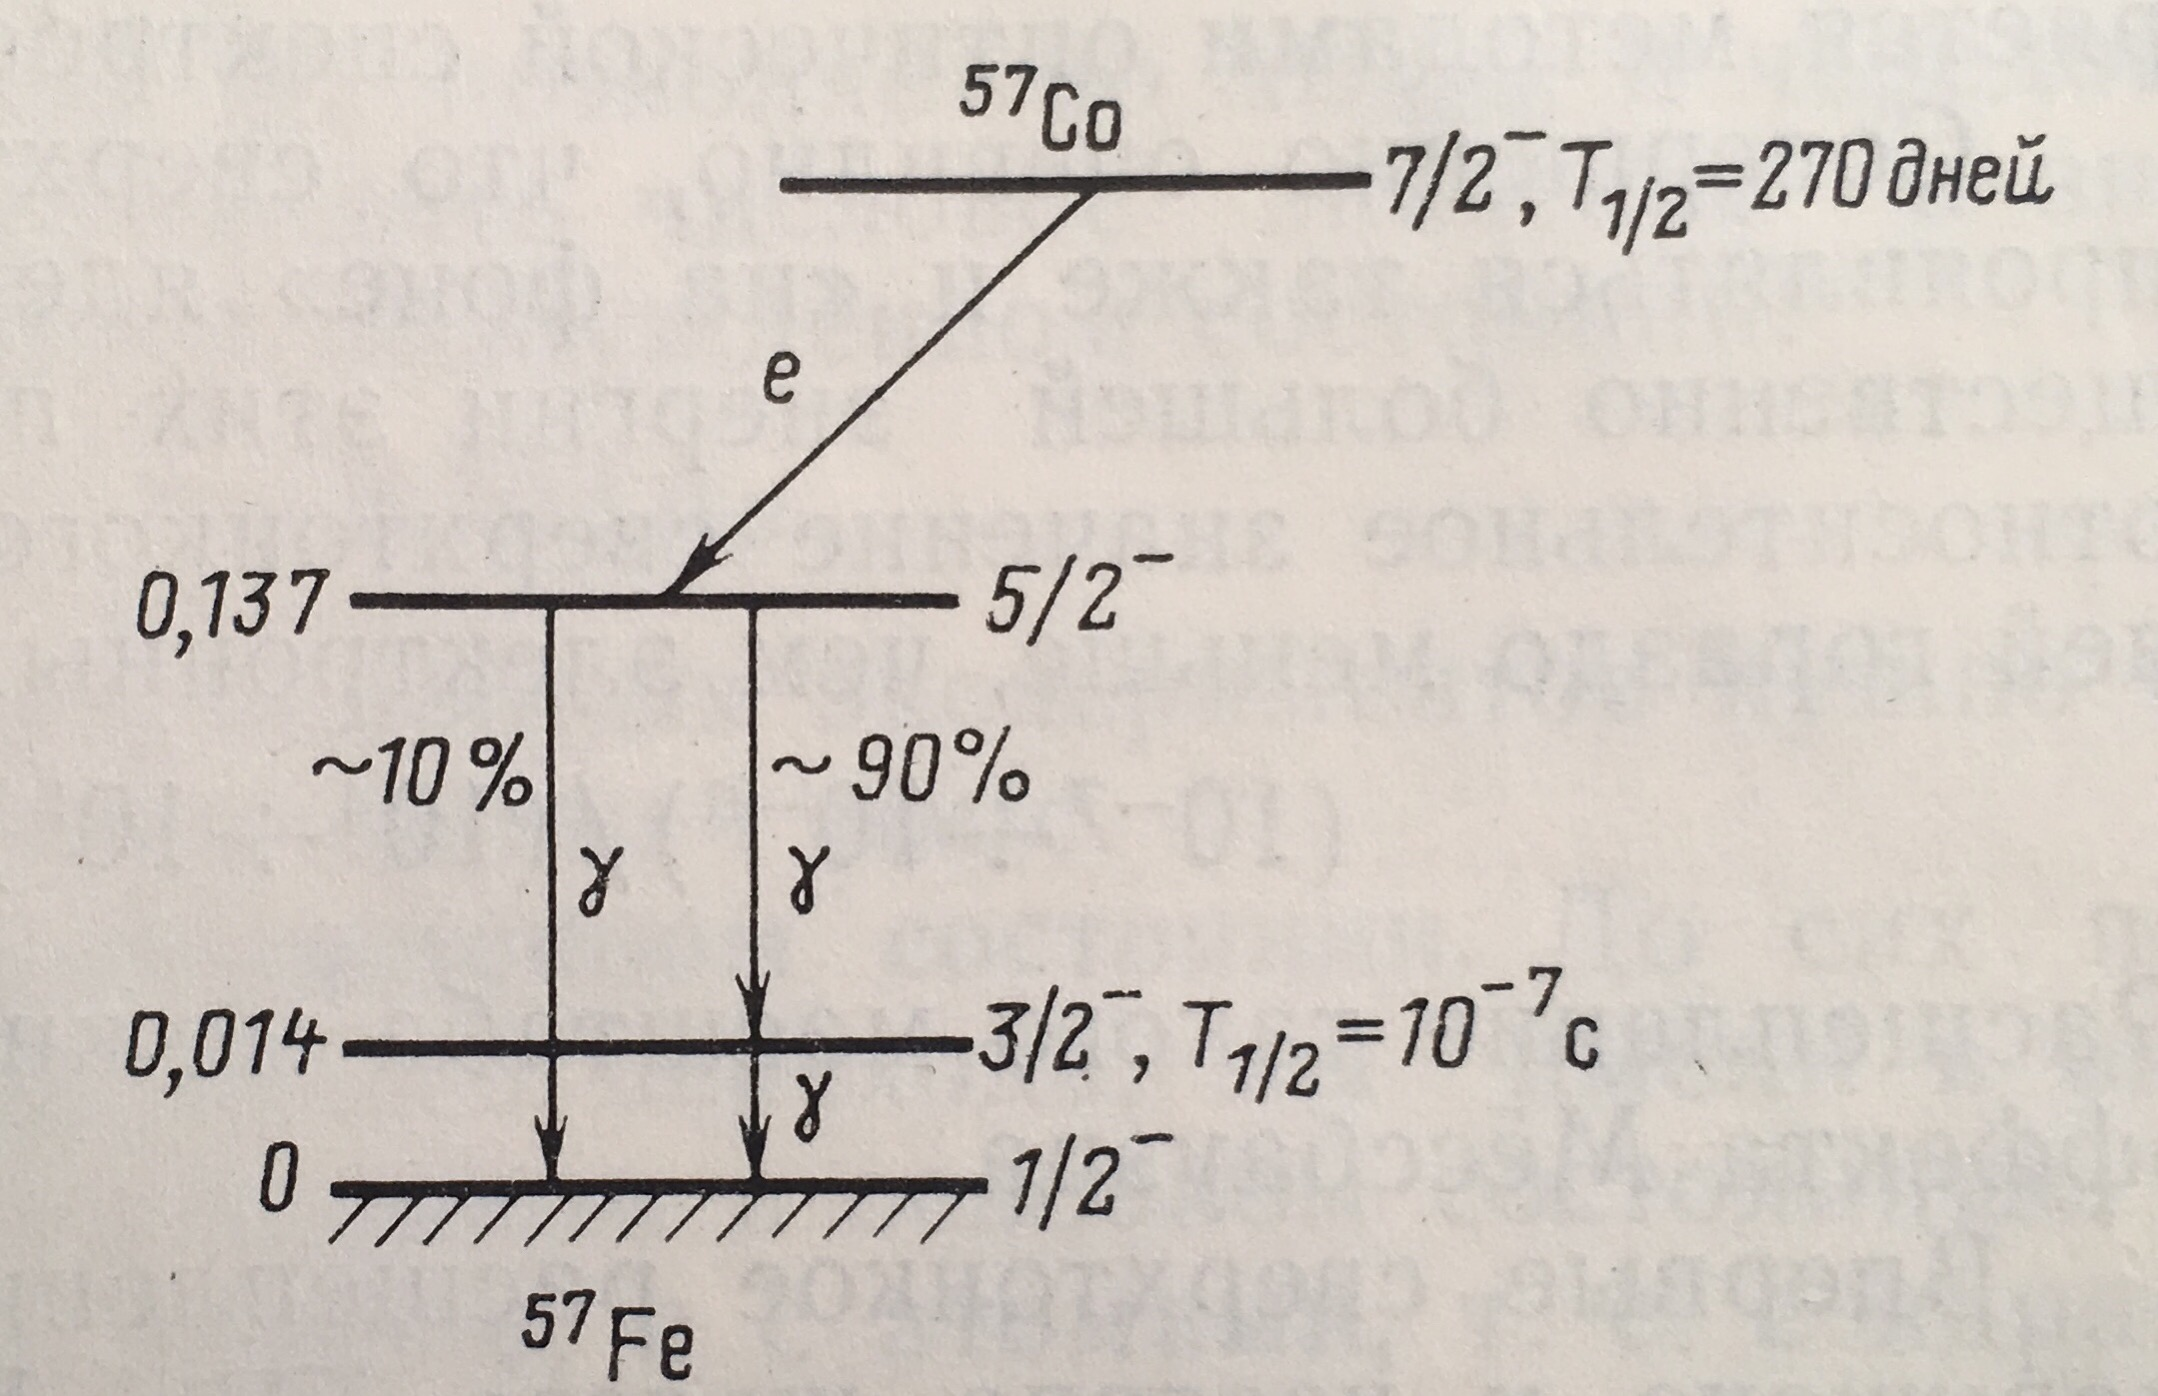
\includegraphics[scale=0.05]{d.jpg}}
\caption{$^{57}Fe$}
\label{fig:image}
\end{figure}

\indent Следовательно, основное состояние должно расщепляться на два подуровня со значениями m = +1/2 и m = -1/2, а возбужденное - на четыре подуровня со значениями m, равными +3/2, +1/2, -1/2, -3/2. Между ними возможны шесть переходов, разрешенных правилами отбора ($\Delta m = 0, \pm 1$).

\begin{figure}[h]
\center{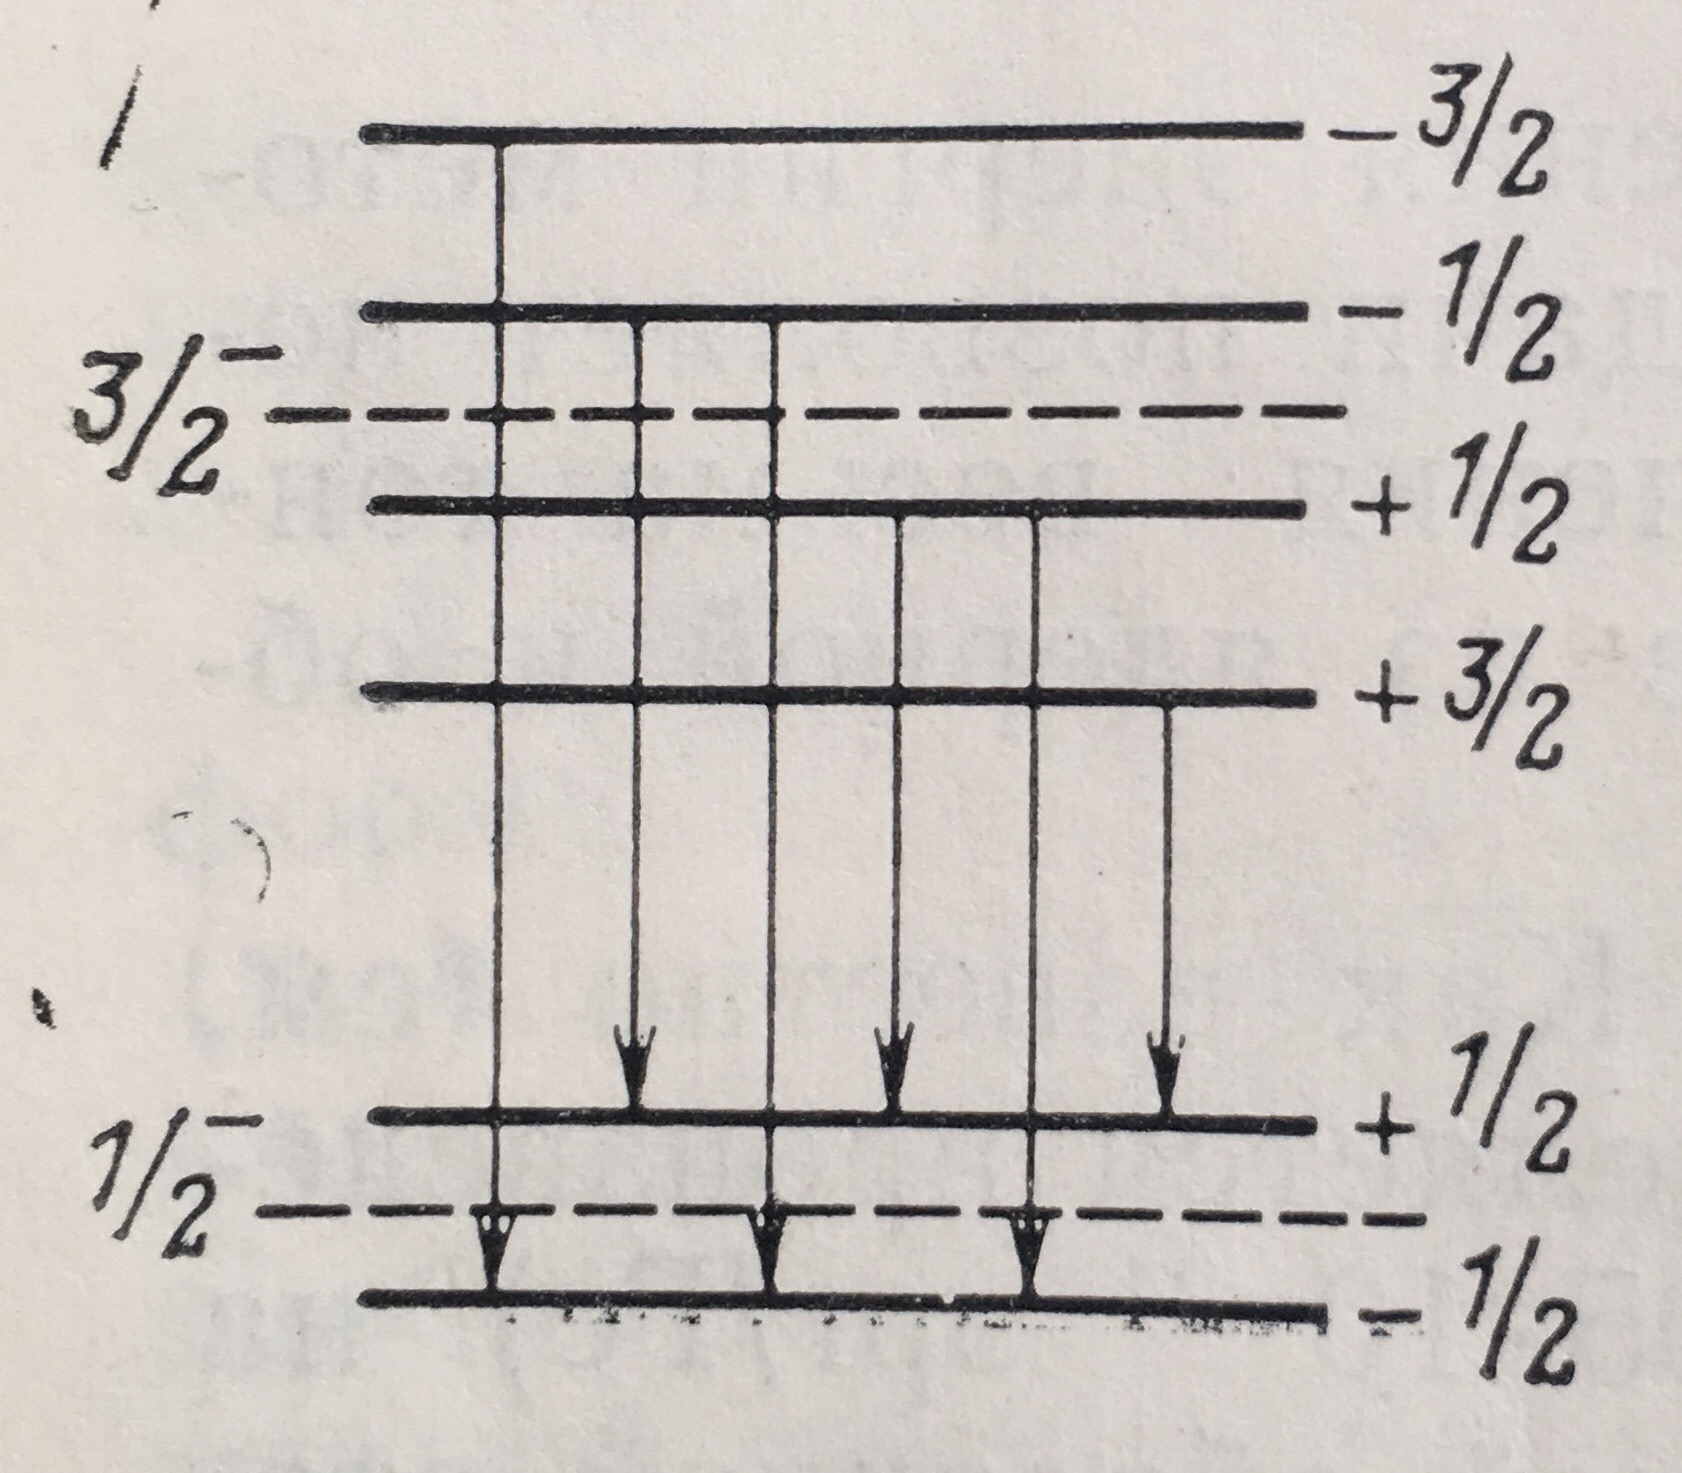
\includegraphics[scale=0.05]{e.jpg}}
\caption{Переходы}
\label{fig:image}
\end{figure}

\indent Такую структуру подуровней, вообще говоря, имеют как ядра-излучатели, так и ядра-поглотители. Поэтому картина зависимости резонансного поглощения от скорости движения источника должна быть очень сложной. Для её упрощения ядра излучателей были включены в диамагнитную решетку из нержавеющей стали. В этом случае для них сверхтонкое расщепление отсутствует и число минимумов на экспериментальной мёссбауэровской кривой совпадает с числом переходов в ядре поглотителе $^{57}Fe$ (Рис. 6). 

\begin{figure}[h]
\center{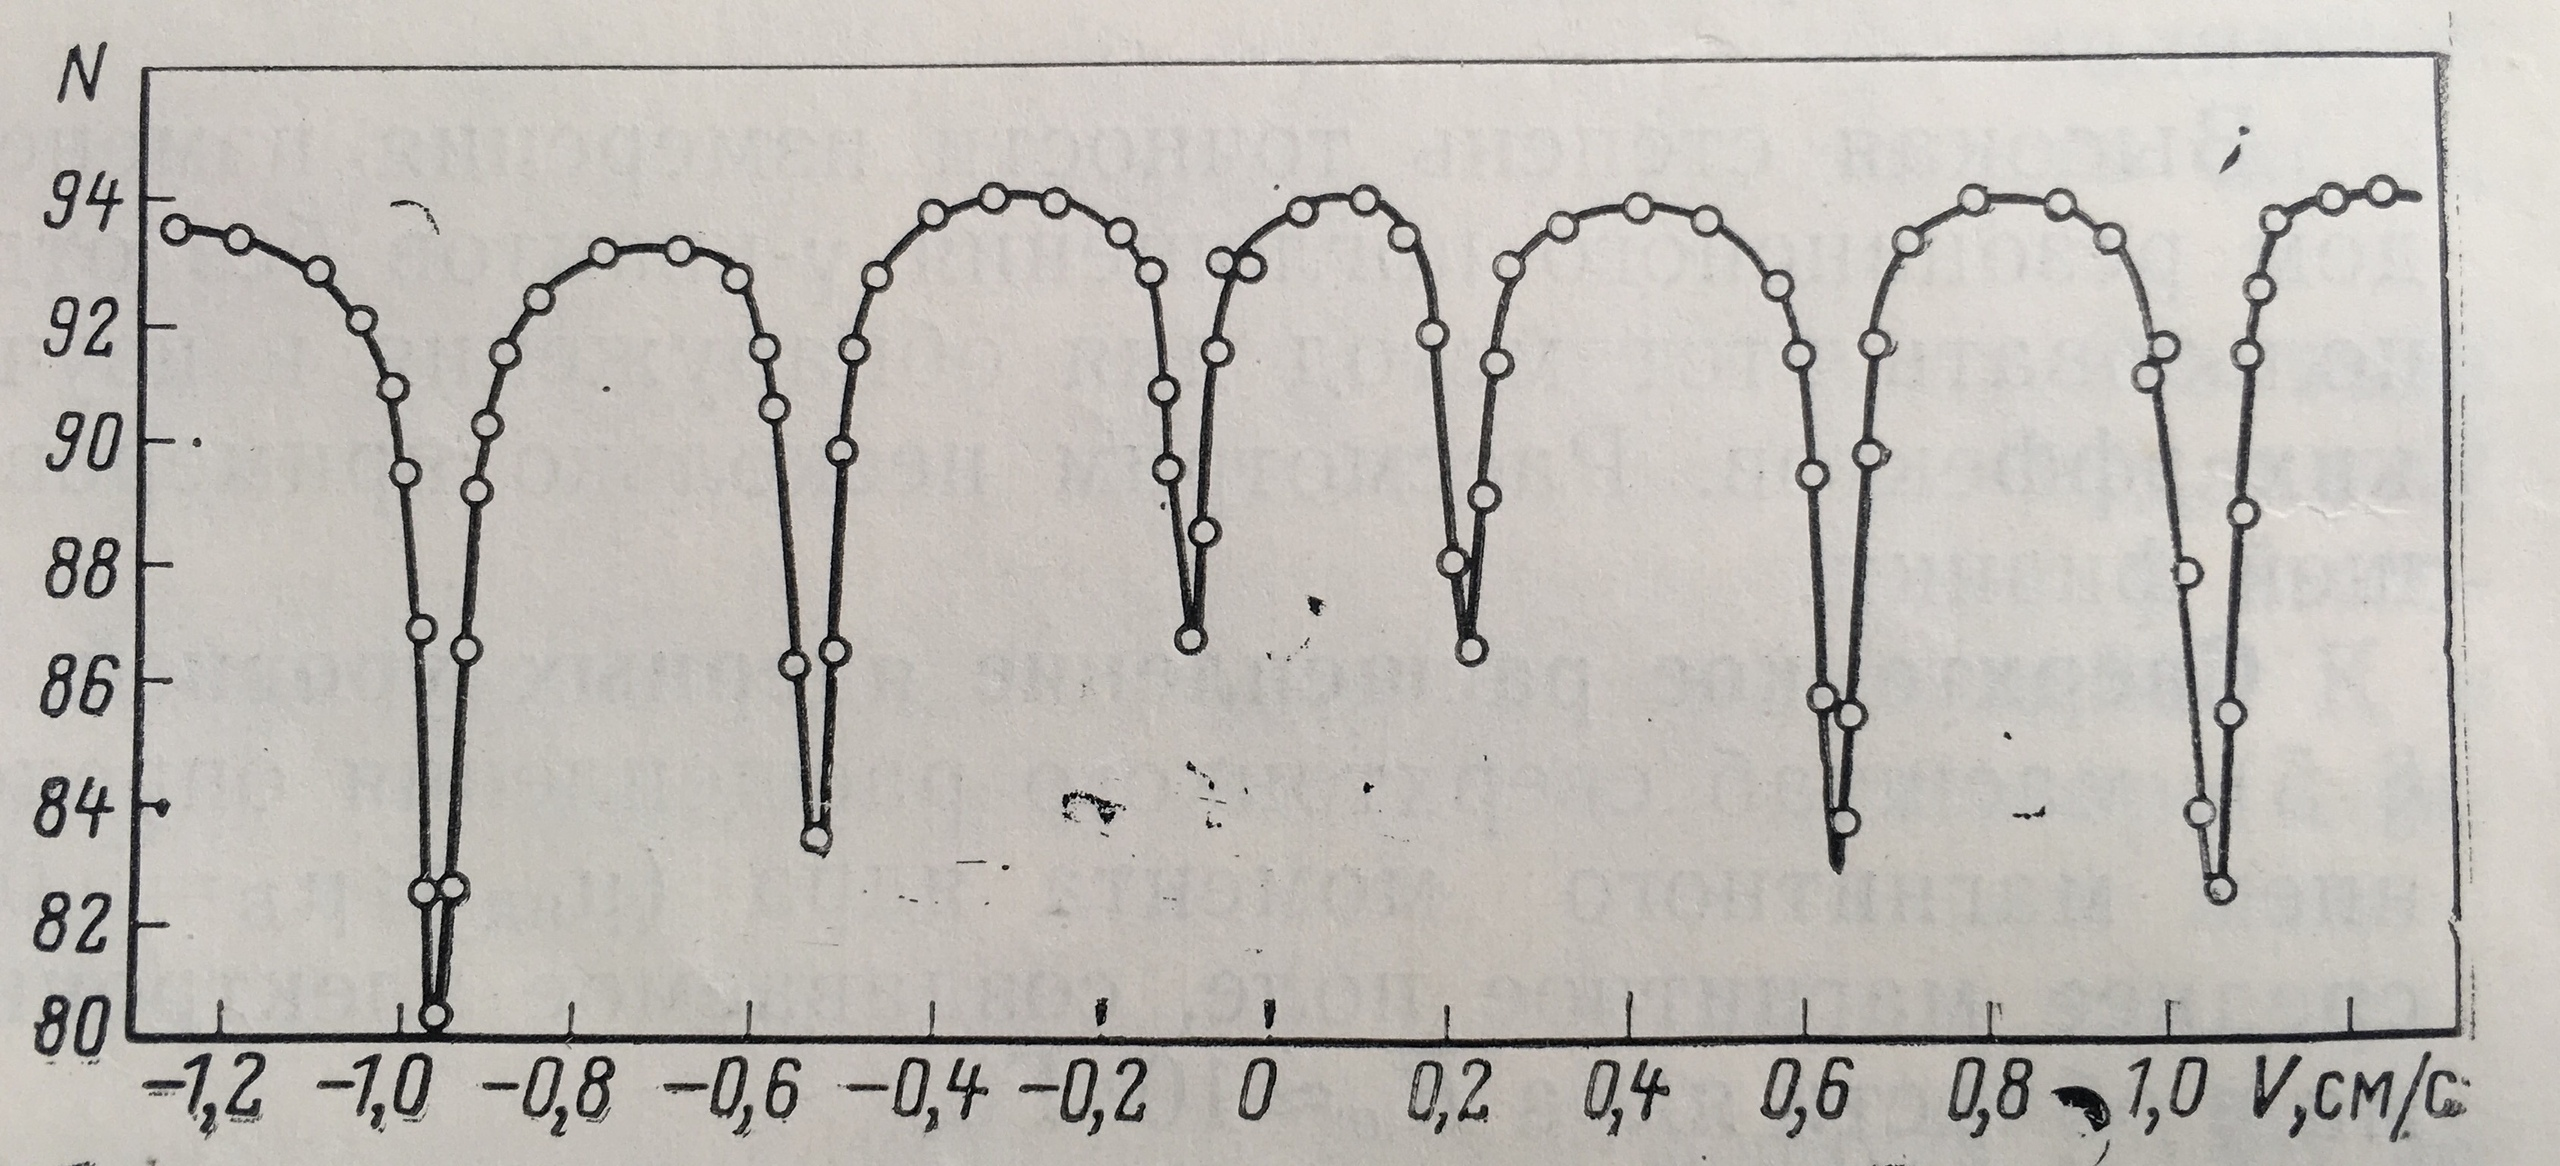
\includegraphics[scale=0.05]{f.jpg}}
\caption{Экспериментальная кривая}
\label{fig:image}
\end{figure}

\indent Расшифровка экспериментальной кривой позволяет вычислить расщепление для основного $\Delta E_{ground}$ и возбужденного $\Delta E_{excited}$ состояний $^{57}Fe$ и порядок чередования магнитного квантового числа m для подуровней возбужденного состояния(Рис. 5). Это дает возможность по $\Delta E_{ground}$ и известному значению магнитного момента $^{57}Fe$ в основном состоянии ($\mu_{ground} = 0,09 \hspace{2pt} \mu_{nuc}$) вычислить среднюю энергию напряженности магнитного поля электронов в районе ядра $^{57}Fe$:
$$ \overline{H_e} = 3,33 \cdot 10^5 \hspace{2pt} \Gamma c .$$
\indent В свою очередь найденное $\overline{H_e}$ позволяет по $\Delta E_{excited}$ и чередованию квантового числа m определить числовое значение и знак магнитного момента ядра $^{57}Fe$ в возбужденном состоянии:
$$ \mu_{excited} = - \hspace{1pt} 0,153 \hspace{2pt} \mu_{nuc}$$
\indent Заметим, что для выполнения подобных экспериментов нужно перемещать источник со скоростью около 1 мм/с.

\subsection{Оценка радиуса ядра в возбужденном состоянии}
\hspace{12pt} До сих пор, говоря об энергии мёссбауэрского перехода, мы имели в виду разность энергий ядра в возбужденном и основном состояниях. Но опыты ставятся не с голыми ядрами,а с атомами, т.е. с ядрами, окруженными электронами. Взаимодействие ядра с электронной оболочкой приводит к сдвигу как ядерных, так и электронных уровней (подобно тому, как сверхтонкое расщепление проявляется как для электронных, так и для ядерных уровней). Величина этого сдвига $\delta E$ зависит от энергии связи электронов с ядром, которая определяется плотностью электронов в области ядра e|$\psi$(0)|$^2$, зарядом ядра Ze и его радиусом R, 
$$ \delta E = (2\pi/5)Ze^2|\psi(0)|^2R^2.$$
\indent Если размеры ядра в основном и возбужденном состояниях различны ($R_{ground} \neq R_{excited}$), сдвиги энергии основного и возбужденного состояний ядра также будут различны $\delta E_{ground} \neq \delta E_{excited}$. Разность этих величин $\Delta E$ и дает поправку к энергии перехода E:
$$ E^{\prime} = E + \Delta E , \hspace{50pt} (1)$$
где ${где} \Delta E = \delta E_{excited} - \delta E_{ground} = (2\pi/5)Ze^2|\psi(0)|^2(R^2_{excited} - R^2_{ground}).$
\\
\indent Если атомы излучатели и поглотители одинаковы, то эта поправка для обоих атомов будет также одинакова ($\Delta E_{em} = \Delta E_{abs}$) и не приведет к расстройке резонанса. Однако если химический состав излучателя и поглотителя различен (при одинаковых ядрах), то из-за различия в энергии связи электронов с ядром-излучателем и ядром-поглотителем (разные электронные оболочки дают $|\psi(0)|^2_{em} \neq |\psi(0)|^2_{abs}$ сдвиги ядерных уровней излучателя и поглотителя будут различны ($\Delta E_{em} \neq \Delta E_{abs}$). Это приводит к различию в исправленных энергиях перехода $E^{\prime}$ и излучателя $E^{\prime}_{em}$ и поглотителя $E^{\prime}_{abs}$. Разность $E^{\prime}_{abs} - E^{\prime}_{em}$ называется химическим или изомерным сдвигом уровней ядра: 
$$ \Delta E_{chem} = E^{\prime}_{abs} - E^{\prime}_{em} = \Delta E^{\prime}_{abs} - \Delta E^{\prime}_{em} $$
\indent В соответствие с формулой (1) химический сдвиг
$$ \Delta E_{chem} = (2\pi/5)Ze^2(|\psi(0)|^2_{abs} - |\psi(0)|^2_{em})\{R^2_{excited} - R^2_{ground}\}.$$
\indent Выражение, стоящее в круглых скобках, в отдельных случаях (при некоторых допущениях) можно вычислить. Поэтому измерение $\Delta E_{chem}$ позволяет оценить радиус ядра в возбужденном состоянии.
\\
\indent Химический сдвиг очень мал ($\Delta E_{chem} \approx 10^{-7} \hspace{2pt} eV; \Delta E/E = 10^{-12}$), но вполне измерим мёссбауэровским методом. Измерения показали, что ядро в возбужденном состоянии может иметь как большие, так и меньшие размеры по сравнению с основным состоянием:
$$ R_{excited}(^{57}Fe) < R_{ground}(^{57}Fe) - 0,1\%.$$
$$ R_{excited}(^{119}Sn) < R_{ground}(^{119}Sn) - 0,01\%.$$
\indent Для проведения подобных измерений необходимы доплеровские скорости около 0,1 мм/с.

\subsection{Измерение красного смещения в лабораторных условиях}
\hspace{12pt} Еще меньшие скорости (около 1 мм/c) потребовались для проверки в лабораторных условиях одного из предсказаний общей теории относительности Эйнштейна. Согласно ОТО $\gamma$-квант с энергией $E_{\gamma}$ должен вести себя в гравитационном поле, как частица с гравитационной массой $m = E_{\gamma} / c^2$. Двигаясь (падая) вдоль силовых линий гравитационного поля, $\gamma$-квант должен приобретать энергию $\Delta E = mgH = (E_{\gamma} / c^2)gH$, где $g$ - ускорение силы тяжести, $H$ - пройденный путь. Его частота при этом возрастает на
$$ \Delta \nu = (E_{\gamma}/hc^2)gH $$
(синее смещение).
\indent Наоборот, при движении против гравитационного поля (вверх) $\gamma$-квант должен терять энергию. Соответственно его частота будет уменьшаться (красное смещение). Относительное изменение энергии очень мало, и при $H$ = 1 м
$$ \Delta E/E = gH/c^2 = 9,81/9\cdot 10^{16} \approx 10^{-16} .$$
\indent Опыт был выполнен в 1959 г. Паундом и Ребкой в башне Гарвардского университета высотой 22,6 м. При таком пролетном пути $\gamma$-кванта относительное изменение энергии составило $\Delta E/E \approx 2,5 \cdot 10^{-15}$, что примерно в $1,5 \cdot 10^{2}$ меньше значения $\Gamma/E \approx 3 \cdot 10^{-13}$ для использованного в опыте изотопа $^{57}Fe$. Таким образом, для надежного обнаружения эффекта необходимо измерять энергию с абсолютной погрешностью $10^{-3} \Gamma \approx 5 \cdot 10^{-12} \hspace{2pt} eV$ и с относительной $\Delta E/E \approx 5 \cdot 10^{-16}$. Такая точность потребовала специальных условий проведения эксперимента (гелиевая среда между излучателем и поглотителем, контроль температуры, защита от вибраций). Легковидеть, что для компенсации измеряемого смещения необходима ничтожная доплеровская скорость, примерно равная 0,75 мм/с. Она была получена с помощью гидраврического устройства с двумя поршнями разных диаметров, меньший из которых приводился в движение часовым механизмом. Для увеличения чувствительности метода в более позднем (1965 г.) опыте Паундаи Снайдера измерение поглощения производилось на наиболее крутых участка резонансной кривой. Для этого скорость излучателя периодически модулировалась в необходимых пределах $\vartheta_{0} \pm \Delta \vartheta$ пьезоэлектрическим вибратором. Результаты измерений согласуются с предсказаниями ОТО. Любопытно отметить, что зарегистрированный земной эффект в $10^{9}$ раз меньше солнечного эффекта, измеряемого астрофизическими методами.

\pagebreak
\Huge\textbf{Литература}
\\
\\
\indent\large 1. Мухин К.Н. Экспериментальная ядерная физика: Учебник для вузов. В 2-х т. Т.1. Физика атомного ядра. - 4-е изд., перераб. и доп. - Москва : Энергоатомиздат, 1983. - 616 с.
\\
\\
\indent\large 2. Инжечик Л.В. Эффект Мёссбауэра и его применения: учебно - методическое пособие. - Москва : МФТИ, 2001. - 28 с.
\\
\\
\indent\large 3. Сивухин Д.В. Общий курс физики. Учеб. пособие : Для вузов. В 5т. Т 5. Атомная и ядерная физика. - 2 - е изд., стереот. - Москва : ФИЗМАТЛИТ; Изд-во МФТИ, 2002. - 784 с.



\end{document}
